\section{Step 2: Mesh}
\label{sec:mesh}

The mesh is made in Ansys Meshing 2024~R2. Close to the two walls it has thin quadrilateral inflation
layers to capture the boundary layer; the rest of the domain is filled with triangles, made smaller
along the nose and at the tip (Figure~\ref{fig:mesh}).

\subsection{Steps}

\begin{enumerate}
\item Open the \gui{Mesh} cell. In \gui{Mesh}\then\gui{Details}: \gui{Physics Preference} = CFD,
\gui{Solver Preference} = Fluent, \gui{Element Order} = Linear, \gui{Element Size} = \SI{0.05}{m},
\gui{Growth Rate} = 1.1, \gui{Smoothing} = High.
\item \gui{Insert}\then\gui{Method} on the surface: triangles. A quadrilateral-dominant fill failed on
this surface.
\item \gui{Insert}\then\gui{Sizing} on edges: \zone{wall\_nose} \SI{1}{mm}; \zone{wall\_body}
\SI{1}{mm} with \gui{Bias Type} towards the shoulder and \gui{Bias Factor} = 3, so the cells are small at
the shoulder and grow towards the outlet.
\item \gui{Insert}\then\gui{Sizing} on the surface, \gui{Type} = \gui{Sphere of Influence}: centre at
the origin (the tip), radius \SI{15}{mm}, element size \SI{0.2}{mm}.
\item \gui{Insert}\then\gui{Inflation} on the surface, boundary = \zone{wall\_nose} and
\zone{wall\_body}: \gui{Inflation Option} = \gui{First Layer Thickness}, first layer
\SI{1}{\micro m}, 45 layers, growth rate 1.2, \gui{Collision Avoidance} = \gui{Layer Compression}.
\item \gui{Generate}, then look at the quality: \gui{Mesh}\then\gui{Quality}\then\gui{Mesh Metric} =
\gui{Skewness}, then \gui{Orthogonal Quality} (Section~\ref{sec:quality}). Close Meshing and
\gui{Update} the Mesh cell so that Fluent receives the mesh with the named selections.
\end{enumerate}

\checkstep{Maximum skewness below 0.95 and minimum orthogonal quality well above 0.01; in Fluent,
\gui{Domain}\then\gui{Mesh}\then\gui{Check} passes with no negative volumes. The study-A mesh has
169\,674 cells (Table~\ref{tab:mesh}).}

\begin{table}[H]
\centering
\caption{Study-A mesh.}
\label{tab:mesh}
\small
\begin{tabular}{@{}ll@{}}
\toprule
Cells & 169\,674 \\
Faces / nodes & 312\,923 / 143\,250 \\
Faces on \zone{wall\_nose} / \zone{wall\_body} & 639 / 1889 \\
Faces on \zone{axis} / \zone{inlet} / \zone{farfield} / \zone{outlet} & 205 / 72 / 121 / 138 \\
\midrule
Maximum skewness (Meshing) & 0.92 \\
Minimum orthogonal quality (Meshing / Fluent) & 0.237 / 0.077 \\
Maximum aspect ratio & 1660 (first inflation layer at the shoulder) \\
Fluent mesh check & passed, no negative volumes \\
\bottomrule
\end{tabular}
\end{table}

\begin{figure}[H]
\centering
\begin{subfigure}[t]{0.49\linewidth}
\centering
\shot{mesh_1_full}{whole domain}
\caption{Whole domain.}
\end{subfigure}\hfill
\begin{subfigure}[t]{0.49\linewidth}
\centering
\shot{mesh_2_nose}{nose and shoulder}
\caption{Nose and shoulder.}
\end{subfigure}

\medskip
\begin{subfigure}[t]{0.49\linewidth}
\centering
\shot{mesh_3_tip}{tip, about 20 mm window}
\caption{Tip, about \SI{20}{mm} window: inflation layers around the rounded tip.}
\label{fig:mesh-tip}
\end{subfigure}\hfill
\begin{subfigure}[t]{0.49\linewidth}
\centering
\shot{mesh_4_inflation}{inflation layers at the shoulder, about 5 mm window}
\caption{Inflation layers at the shoulder, about \SI{5}{mm} window.}
\end{subfigure}
\caption{Study-A mesh, as read by Fluent.}
\label{fig:mesh}
\end{figure}

\subsection{Why these sizes}

\paragraph{First cell height.} SST is solved down to the wall, without wall functions, so the first cell
must sit in the viscous layer: $y^+ = \rho u_\tau y/\mu \approx 1$. Flat-plate estimate at the shoulder
($x = \SI{0.559}{m}$), with the free stream of Section~\ref{sec:freestream}:
\begin{equation}
\mathrm{Re}_x = \frac{\rho V x}{\mu}, \qquad
C_f \approx 0.026\,\mathrm{Re}_x^{-1/7}, \qquad
u_\tau = V\sqrt{\frac{C_f}{2}}, \qquad
h_1 = \frac{y^+\,\mu}{\rho\,u_\tau}\bigg|_{y^+ = 1}.
\label{eq:y1}
\end{equation}
This gives $h_1 = 1.38$, 1.16 and \SI{1.02}{\micro m} at $M = 0.95$, 1.2 and 1.47, so one mesh with
$h_1 = \SI{1}{\micro m}$ covers all three. Fluent's $y^+$ after the runs stays below 0.71 on the nose and
0.30 on the cylinder (Figure~\ref{fig:yplus}).

\begin{figure}[H]
\centering
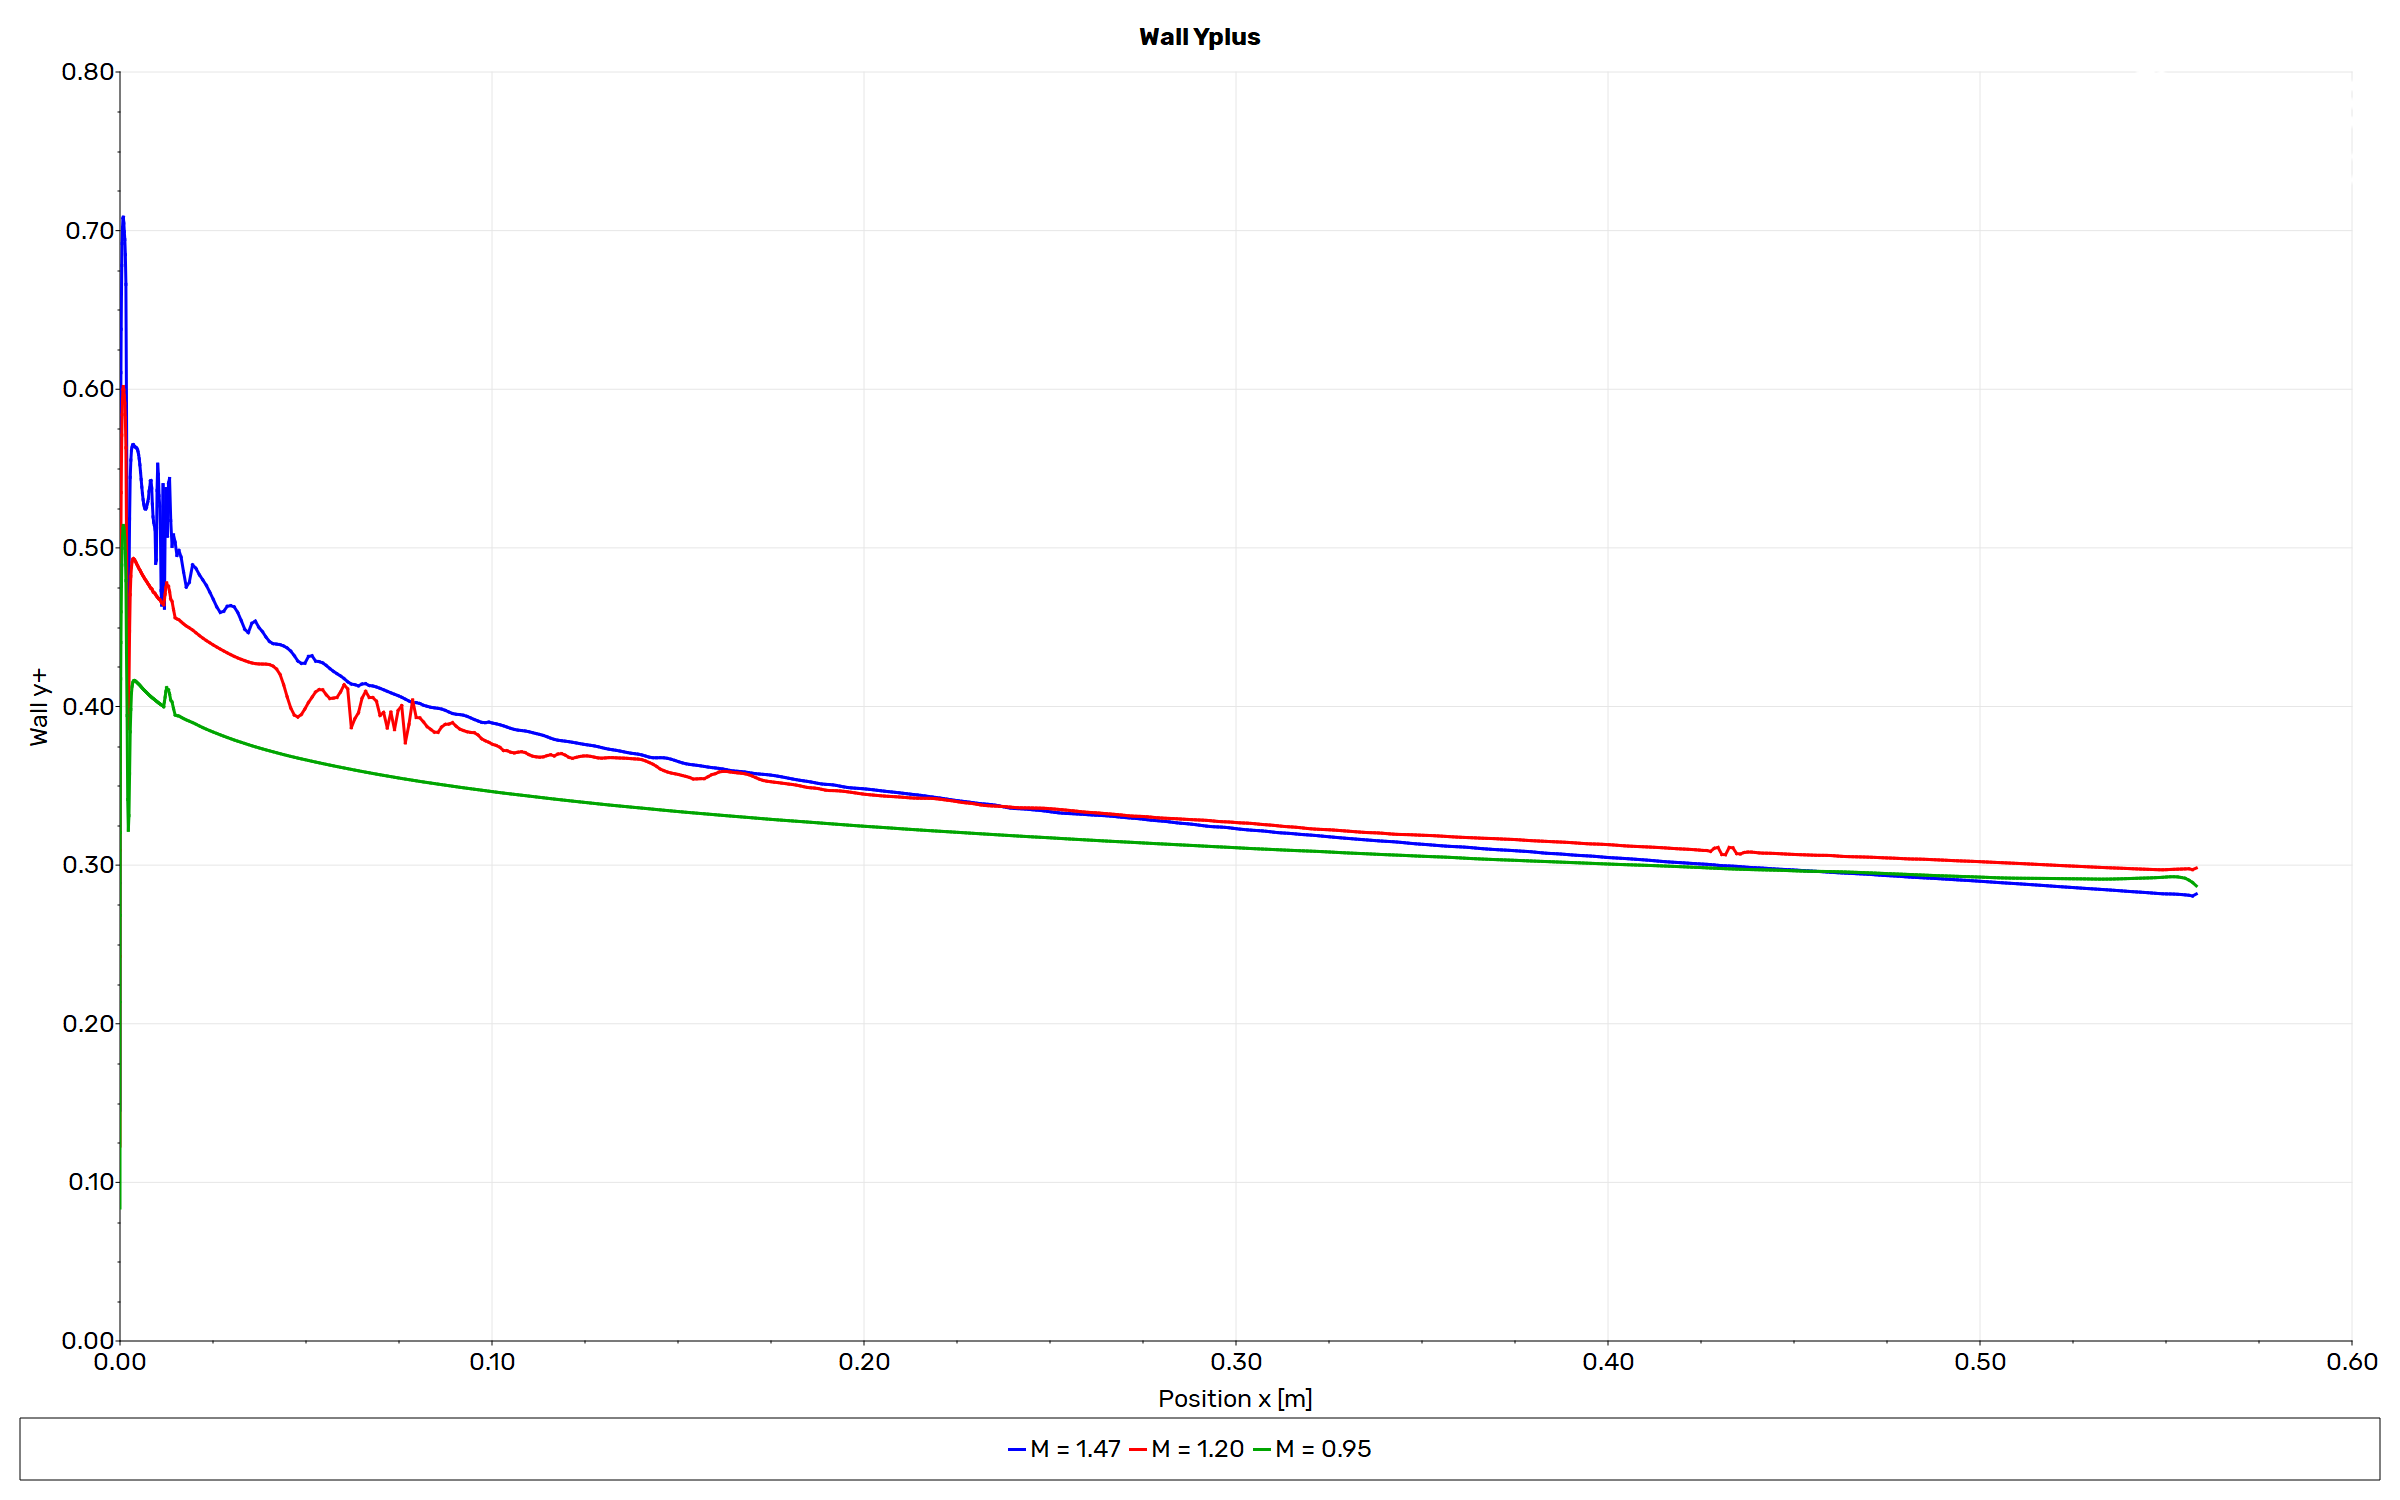
\includegraphics[width=0.9\linewidth]{fluent_yplus_all}
\caption{Wall $y^+$ along \zone{wall\_nose} at the three Mach numbers (Fluent XY plot). It stays below
1 everywhere, as Equation~\eqref{eq:y1} intended.}
\label{fig:yplus}
\end{figure}

\paragraph{Inflation thickness.}
\begin{equation}
H = h_1\,\frac{1.2^{45} - 1}{1.2 - 1} = \SI{18.3}{mm},
\qquad h_{45} = h_1 \times 1.2^{44} = \SI{3.05}{mm}.
\end{equation}
The boundary layer at the shoulder is $\delta \approx 0.37\,x\,\mathrm{Re}_x^{-1/5} = 7.5$--\SI{8.0}{mm},
so it lies entirely inside the inflation layers.

\paragraph{Tip.} The tip arc $\pi r_n/2 = \SI{7.07}{mm}$ gets about 35 cells of \SI{0.2}{mm}. This is where
the bow shock forms and the wall pressure changes fastest (Figure~\ref{fig:cp}).

\subsection{Mesh quality}
\label{sec:quality}

\begin{table}[H]
\centering
\caption{Mesh quality of study~A (\gui{Mesh}\then\gui{Quality}\then\gui{Mesh Metric} in Meshing, mesh check in Fluent).}
\label{tab:quality}
\small
\begin{tabularx}{\linewidth}{@{}l>{\raggedright\arraybackslash}X>{\raggedright\arraybackslash}p{2.3cm}>{\raggedright\arraybackslash}p{3.3cm}@{}}
\toprule
Metric & Meaning & Limit & Study A \\
\midrule
Skewness & how far the cell angles are from the ideal shape (0 = perfect, 1 = flattened cell) & maximum $< 0.95$ & 0.92, acceptable \\
Orthogonal quality & how well each face lines up with the line between the two cell centres (1 = perfect, 0 = worst) & minimum $> 0.01$ (Fluent) & 0.237 (Meshing), 0.077 (Fluent) \\
Aspect ratio & cell length / cell height & none for inflation layers & 1660, first layer at the shoulder \\
\bottomrule
\end{tabularx}
\end{table}

\begin{table}[H]
\centering
\caption{How Ansys Meshing rates skewness and orthogonal quality.}
\label{tab:bands}
\small
\begin{tabular}{@{}lcccccc@{}}
\toprule
Skewness & 0--0.25 & 0.25--0.50 & 0.50--0.80 & 0.80--0.94 & 0.95--0.97 & 0.98--1 \\
 & excellent & very good & good & acceptable & bad & unacceptable \\
\midrule
Orthogonal quality & 0--0.001 & 0.001--0.14 & 0.15--0.20 & 0.20--0.69 & 0.70--0.95 & 0.95--1 \\
 & unacceptable & bad & acceptable & good & very good & excellent \\
\bottomrule
\end{tabular}
\end{table}

\begin{itemize}
\item The worst cells are near the outlet, where the last inflation layers on \zone{wall\_body} meet the
triangles, \SI{1.4}{m} behind the nose; around the nose the cells are close to ideal
(Figure~\ref{fig:mesh-tip}).
\item A bias factor of 10 on \zone{wall\_body} stretched those cells to a skewness of 0.985 (38 cells,
``unacceptable''); a bias factor of 3 brought the maximum down to 0.92.
\item Long, thin first layers (aspect ratio about 1000) are normal for $y^+ \approx 1$: across the
boundary layer the velocity changes about a thousand times faster than along the wall.
\end{itemize}
